\documentclass{notes}
\usepackage[makeroom]{cancel}

\author{Ritchie Cai, Matthew Mosley \& Corey Higgins}
\title{Inverted Pendulum Summary}

\begin{document}
\maketitle 
\section{Idea}
For the past few weeks, we have been designing a system that consists of an inverted pendulum on two wheels. This design is constructed by using the programmable BRIC from a LEGO Mindstorms EV3 set and additional LEGO pieces to physically construct it (seen in photos from modeling document). The overall goal of the system is to have the two wheels balance the pendulum in an upright, vertical position and to continue doing so after any slight disturbances that may offset the inverted pendulum by a relatively small angle (this assumed small angle comes into play in design calculations). 

\section{Implementation}
The implementation of our controller is written in Java running on top of LeJOS which is a variance of the embedded Linux running embedded JVM. The Java interface allows us to control motors' acceleration and speed. In addition to motor we also have two gyro sensors, one is used to measuring the incline angle of the pendulum, the other one is used to measure the rate of change of the incline angle. The sensors prove to be a critical aspect of how we approached the math in the next, Analysis, section. Since we have control over acceleration and velocity of the motors driving the wheels, we would have to implement a design with an acceleration input. Then, our only way of effectively measuring the changing angle of the pendulum was through use of the two gyro sensors. So the angle would be our only output of our system in our design.

\section{Analysis}  
The designing process began with observing and analyzing the physics behind our system. Friction was ignored as the design intended to use a PID controller to cancel out friction's effect. For ease of calculation, we approximated our pendulum offset angles to be very small where sin($\theta$)= $\theta$, and cos($\theta$)= 1. As seen in the modeling document, we were able to derive the governing equations of motion behind our design. As expected, we observed that our inverted pendulum transfer function was unstable, which is clearly indicated by a pole existing in the positive, right half plane in our pole-zero diagram on the modeling document. This result made a controlling mechanism a necessity in order to gain stability for our system. As for the controller used, a simple PID controller was chosen along with negative feedback through the use of a LEGO Mindstorms EV3 gyro sensor. The unstable transfer function that represents the inverted pendulum system is as follows:
\[
  T(s) = \dfrac{\Theta}{U} = \dfrac{M+m}{m}\dfrac{\frac{2}{L}}{s^2-\frac{2g}{L}}
\]
This  transfer was then incorporated into the block diagram and then the transfer function that governed the entire system is represented by:

Then the overall block diagram with negative feedback from gyro sensor looks like:
\begin{figure}[!h]
  \begin{center}
    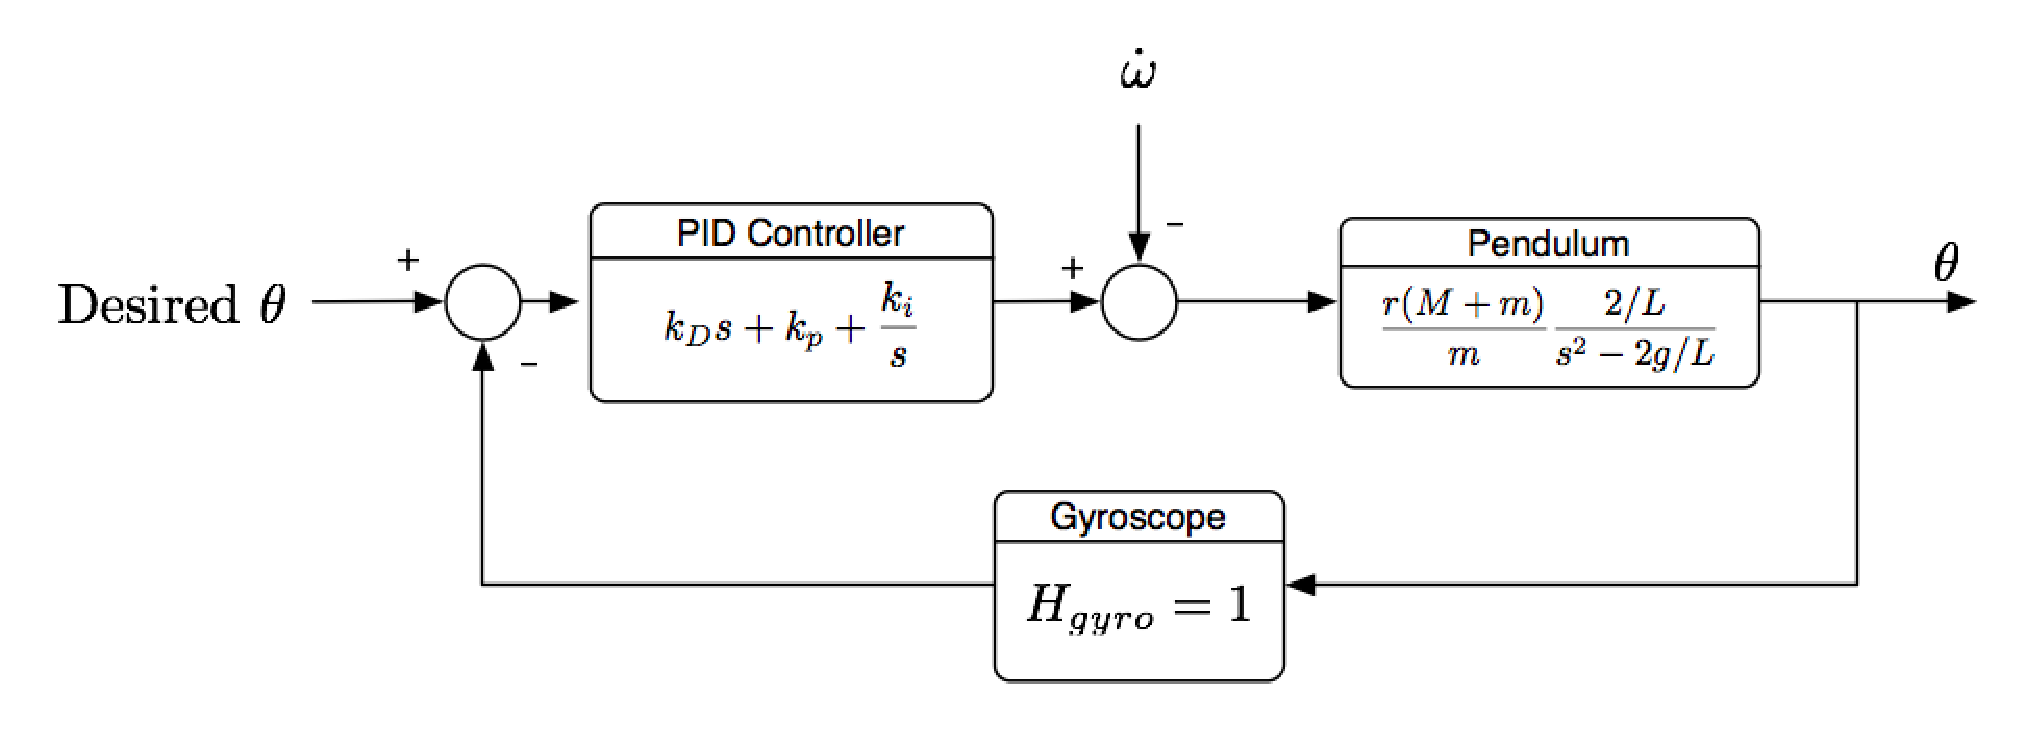
\includegraphics[width=5 in]{pics/Block_Diagram_2.eps}
  \end{center}
  \caption{Block diagram for our system}
  \label{fig:block_diagram}
\end{figure}

\section{Design Specifications}
We then went on to tune our system's parameters, $K_p$, $K_i$, and $K_d$, to optimize correction to any disturbance. In fact, the overall settling time simulated on MATLAB came out be 1.22 seconds. 
The first transfer function can be described as having acceleration inputs and an angle theta, for the pendulum position, being the observed output. The design should adhere to the following specifications: settling time should be very responsive, pendulum angle theta never rotating beyond 20 degrees or so, and the steady state error should be small as well.  

 \section{Results}
The most difficult part of the design procedure was
   
\end{document}